% IMT 583 GP4 — Meridian Health LMS Project Plan
% LaTeX report template based on the visual conventions of the supplied exemplar.
% Compile with: pdflatex meridian_gp4_template.tex
% Run pdflatex twice to populate the table of contents and cross-references.

\documentclass[11pt,letterpaper]{article}

% ---------- Page geometry and typography ----------
\usepackage[letterpaper,margin=0.78in,headheight=16pt,headsep=0.22in,footskip=0.38in]{geometry}
\usepackage[T1]{fontenc}
\usepackage{lmodern}
\usepackage{microtype}
\usepackage{setspace}
\setstretch{1.04}
\usepackage{ragged2e}

% ---------- Color and section styling ----------
\usepackage[table,dvipsnames]{xcolor}
\definecolor{MeridianPurple}{HTML}{4B2E83}
\definecolor{MeridianLavender}{HTML}{EEEAF4}
\definecolor{MeridianPale}{HTML}{F7F5FA}
\definecolor{MeridianGray}{HTML}{555555}
\definecolor{MeridianRule}{HTML}{777777}

\usepackage{titlesec}
\titleformat{\section}
  {\Large\bfseries\color{MeridianPurple}}
  {\thesection.}{0.55em}{}
\titlespacing*{\section}{0pt}{1.5em}{0.65em}

\titleformat{\subsection}
  {\large\bfseries\color{MeridianPurple}}
  {\thesubsection}{0.55em}{}
\titlespacing*{\subsection}{0pt}{1.15em}{0.4em}

\titleformat{\subsubsection}
  {\normalsize\bfseries\color{MeridianPurple}}
  {\thesubsubsection}{0.55em}{}
\titlespacing*{\subsubsection}{0pt}{0.8em}{0.25em}

% ---------- Tables ----------
\usepackage{array}
\usepackage{tabularx}
\usepackage{booktabs}
\usepackage{longtable}
\usepackage{makecell}
\usepackage{multirow}
\usepackage{colortbl}
\usepackage{ragged2e}

\renewcommand{\arraystretch}{1.22}
\setlength{\tabcolsep}{5pt}
\newcolumntype{Y}{>{\RaggedRight\arraybackslash}X}
\newcolumntype{L}[1]{>{\RaggedRight\arraybackslash}p{#1}}
\newcolumntype{C}[1]{>{\Centering\arraybackslash}p{#1}}

% Use this header row in tabular/tabularx/longtable:
\newcommand{\tableheader}[1]{%
  \rowcolor{MeridianPurple}\color{white}\bfseries #1%
}
% Alternating row colors:
\newcommand{\tablebodycolors}{%
  \rowcolors{2}{MeridianPale}{white}%
}

% ---------- Figures, captions, lists ----------
\usepackage{graphicx}
\usepackage{float}
\usepackage{caption}
\captionsetup{
  font=small,
  labelfont=bf,
  textfont=it,
  justification=centering,
  skip=6pt
}
\usepackage{enumitem}
\setlist[itemize]{leftmargin=1.5em,itemsep=0.22em,topsep=0.3em}
\setlist[enumerate]{leftmargin=1.8em,itemsep=0.28em,topsep=0.3em}

% ---------- Headers and footers ----------
\usepackage{fancyhdr}
\setlength{\headheight}{22pt}
\pagestyle{fancy}
\fancyhf{}
\fancyhead[L]{\small\color{MeridianGray}Meridian Health LMS Implementation}
\fancyhead[R]{\small\color{MeridianGray}Comprehensive Project Plan v1.0}
\fancyfoot[L]{\small\color{MeridianGray}Team [X] \textbar\ IMT 583 GP4}
\fancyfoot[R]{\small\color{MeridianGray}Page \thepage}
\renewcommand{\headrulewidth}{0.35pt}
\renewcommand{\footrulewidth}{0pt}
\renewcommand{\headrule}{\hbox to\headwidth{\color{MeridianRule}\leaders\hrule height \headrulewidth\hfill}}

% ---------- Links and PDF metadata ----------
\usepackage[hidelinks]{hyperref}
\hypersetup{
  pdftitle={Meridian Health LMS Comprehensive Project Plan},
  pdfauthor={IMT 583 GP4 Team}
}

% ---------- Utility commands ----------
\newcommand{\placeholder}[1]{\textit{\color{MeridianGray}[Insert #1]}}

\begin{document}

% ============================================================
% COVER PAGE
% ============================================================
\thispagestyle{empty}
\vspace*{1.05in}

{\large\color{MeridianGray}Meridian Health\par}
\vspace{0.18in}
{\Huge\bfseries\color{MeridianPurple}Learning Management System\par}
\vspace{0.12in}
{\LARGE Comprehensive Project Plan\par}
\vspace{0.55in}

\renewcommand{\arraystretch}{1.45}
\begin{tabularx}{\textwidth}{|L{1.55in}|Y|}
\hline
\rowcolor{MeridianPurple}
\color{white}\bfseries Item & \color{white}\bfseries Detail\\
\hline
Plan version & 1.0 (proposed baseline; subject to required approvals)\\
\hline
Project sponsor & Chief Human Resources Officer (CHRO)\\
\hline
Project manager & [Project Manager / Team] \\
\hline
Planned duration & [Confirm approved start date, end date, and working-day duration]\\
\hline
Related documents & GP1 Project Proposal; GP2 Project Charter and Build vs. Buy Analysis; GP3 Kickoff Presentation\\
\hline
Gantt chart & Submitted separately: [Gantt chart filename; full view and detail views]\\
\hline
Team members & \makecell[l]{Lincoln Brennan; Kyle Chen;\\ Kshitij Dani; Sekoya Kinsey}\\
\hline
\end{tabularx}

\vfill
\begin{center}
{\small\color{MeridianGray}IMT 583 \textbar\ Group Project 4 \textbar\ November 2026}
\end{center}
\clearpage

% ============================================================
% TABLE OF CONTENTS
% ============================================================
\pagenumbering{arabic}
\setcounter{page}{1}
\tableofcontents
\clearpage

% ============================================================
% 1. DETAILED SCOPE STATEMENT
% ============================================================
\section{Detailed Scope Statement}

\subsection{Project scope description}
\placeholder{existing scope description from the Skeleton, preserving its approved wording}.

\subsection{Project deliverables}
% Recommended columns: WBS ID, Deliverable, Description, Acceptance and approval.
\begin{tabularx}{\textwidth}{|L{0.75in}|L{1.55in}|Y|L{1.65in}|}
\hline
\rowcolor{MeridianPurple}
\color{white}\bfseries WBS ID &
\color{white}\bfseries Deliverable &
\color{white}\bfseries Description &
\color{white}\bfseries Acceptance and approval\\
\hline
1.0 & Requirements and Verification Record & \placeholder{deliverable description} & \placeholder{acceptance authority}\\
\hline
2.0 & Vendor Assessment and Selection Record & \placeholder{deliverable description} & \placeholder{acceptance authority}\\
\hline
% Add remaining deliverables from the Skeleton.
\end{tabularx}

\subsection{Features and functionality}
\begin{itemize}
  \item \textbf{Employee accounts and access:} \placeholder{feature description}
  \item \textbf{Centralized training library:} \placeholder{feature description}
  % Add remaining features from the Skeleton.
\end{itemize}

\subsection{Performance requirements (SLAs)}
% Recommended columns: Area, Requirement, Verification and WBS reference.
\begin{tabularx}{\textwidth}{|L{1.25in}|Y|Y|}
\hline
\rowcolor{MeridianPurple}
\color{white}\bfseries Area &
\color{white}\bfseries Requirement &
\color{white}\bfseries Verification and WBS reference\\
\hline
Sign-in response time & \placeholder{measurable target} & \placeholder{verification method and WBS reference}\\
\hline
Concurrent capacity & \placeholder{measurable target} & \placeholder{verification method and WBS reference}\\
\hline
% Add remaining SLA rows.
\end{tabularx}

\subsection{Quality standards}
\placeholder{quality standards statement from the Skeleton}.

\subsection{Project phases and major activities}
% Recommended columns: Phase, Planned dates, Major activities, Completion milestone.
\begin{tabularx}{\textwidth}{|L{1.25in}|L{1.15in}|Y|L{1.55in}|}
\hline
\rowcolor{MeridianPurple}
\color{white}\bfseries Phase &
\color{white}\bfseries Planned dates &
\color{white}\bfseries Major activities &
\color{white}\bfseries Completion milestone\\
\hline
Kickoff and requirements & \placeholder{dates} & \placeholder{activities} & \placeholder{milestone}\\
\hline
% Add remaining phases.
\end{tabularx}

\subsection{Explicitly stated exclusions}
\begin{enumerate}[label=\alph*.]
  \item \textbf{Custom LMS development:} \placeholder{existing exclusion}
  % Add remaining exclusions.
\end{enumerate}

\subsection{Scope baseline}
\placeholder{existing scope baseline text}.

\subsection{WBS reference}
\placeholder{existing WBS reference text}.

\subsection{Scope control process}
\begin{itemize}
  \item \textbf{Verify:} \placeholder{process}
  \item \textbf{Monitor:} \placeholder{process}
  \item \textbf{Prevent scope creep:} \placeholder{process}
  \item \textbf{Control:} \placeholder{process}
\end{itemize}

\subsection{Change request procedure}
\begin{enumerate}
  \item \textbf{Submit:} \placeholder{process}
  \item \textbf{Log:} \placeholder{process}
  \item \textbf{Analyze:} \placeholder{process}
  \item \textbf{Decide:} \placeholder{process}
  \item \textbf{Update and communicate:} \placeholder{process}
  \item \textbf{Implement and close:} \placeholder{process}
\end{enumerate}

% Add the approval-authority table and change-log template from the Skeleton here.

% ============================================================
% 2. WORK BREAKDOWN STRUCTURE
% ============================================================
\clearpage
\section{Work Breakdown Structure}

\subsection{Visual WBS}
% Export the editable WBS diagram to PDF or a high-resolution image.
\begin{figure}[H]
  \centering
  \IfFileExists{figures/meridian_wbs.pdf}{%
    \includegraphics[width=\textwidth,height=0.72\textheight,keepaspectratio]{figures/meridian_wbs.pdf}%
  }{\fbox{\parbox[c][2.0in][c]{0.9\textwidth}{\centering
    WBS figure placeholder. Upload \texttt{figures/meridian\_wbs.pdf}.}}}
  \caption{Work breakdown structure for the Meridian Health LMS implementation.}
  \label{fig:wbs}
\end{figure}

\subsection{WBS dictionary}
\placeholder{Insert the WBS dictionary or a reference to the separately submitted spreadsheet.}
% For a wide dictionary, use landscape pages and longtable.
% Recommended columns: WBS ID/name, Description, Responsible, Effort/duration,
% Dependencies, Required resources, Acceptance criteria.

% ============================================================
% 3. PROJECT SCHEDULE
% ============================================================
\clearpage
\section{Project Schedule}

\subsection{Gantt chart summary}
\placeholder{Insert a readable Gantt chart summary or reference the separately submitted PDF.}
% If included in this report:
% \begin{figure}[H]
%   \centering
%   \includegraphics[width=\textwidth]{figures/meridian_gantt_summary.pdf}
%   \caption{Meridian Health LMS project schedule.}
% \end{figure}

\subsection{Schedule narrative}
\subsubsection{Project duration and end date}
\placeholder{Insert schedule narrative.}

\subsubsection{Critical path analysis and implications}
\placeholder{Insert schedule narrative.}

\subsubsection{Major milestones and their significance}
\placeholder{Insert schedule narrative.}

\subsubsection{Resource loading and allocation strategy}
\placeholder{Identify roles, effort, peaks/over-allocations, leveling or smoothing, critical-path assignments, backups, and contingency actions.}

\subsubsection{Schedule assumptions and constraints}
\placeholder{Insert schedule narrative.}

\subsubsection{Schedule risks and buffer strategy}
\placeholder{Insert schedule narrative.}

\subsubsection{Schedule maintenance and updates}
\placeholder{Insert schedule narrative.}

% ============================================================
% 4. RISK MANAGEMENT PLAN
% ============================================================
\clearpage
\section{Risk Management Plan}

\subsection{Risk management approach}
\subsubsection{Risk identification methodology}
\placeholder{Insert methodology.}

\subsubsection{Risk assessment criteria and scales}
\placeholder{Define probability, impact, scoring, and rating thresholds.}

\subsubsection{Risk monitoring and control process}
\placeholder{Insert monitoring and control process.}

\subsubsection{Risk reporting frequency and format}
\placeholder{Insert reporting process.}

\subsubsection{Risk escalation thresholds}
\placeholder{Insert escalation thresholds.}

\subsection{Risk register}
% The Skeleton requires at least 12 risks.
% This table is intentionally placed on landscape pages in the final document
% if portrait layout makes the response-action column difficult to read.
% Recommended columns: Risk ID, Description, Category, Probability, Impact,
% Score, Response strategy, Specific response action, Owner, Trigger conditions.
\placeholder{Insert risk register with at least 12 risks.}

\subsection{Probability/impact matrix}
\begin{figure}[H]
  \centering
  \IfFileExists{figures/meridian_risk_matrix.pdf}{%
    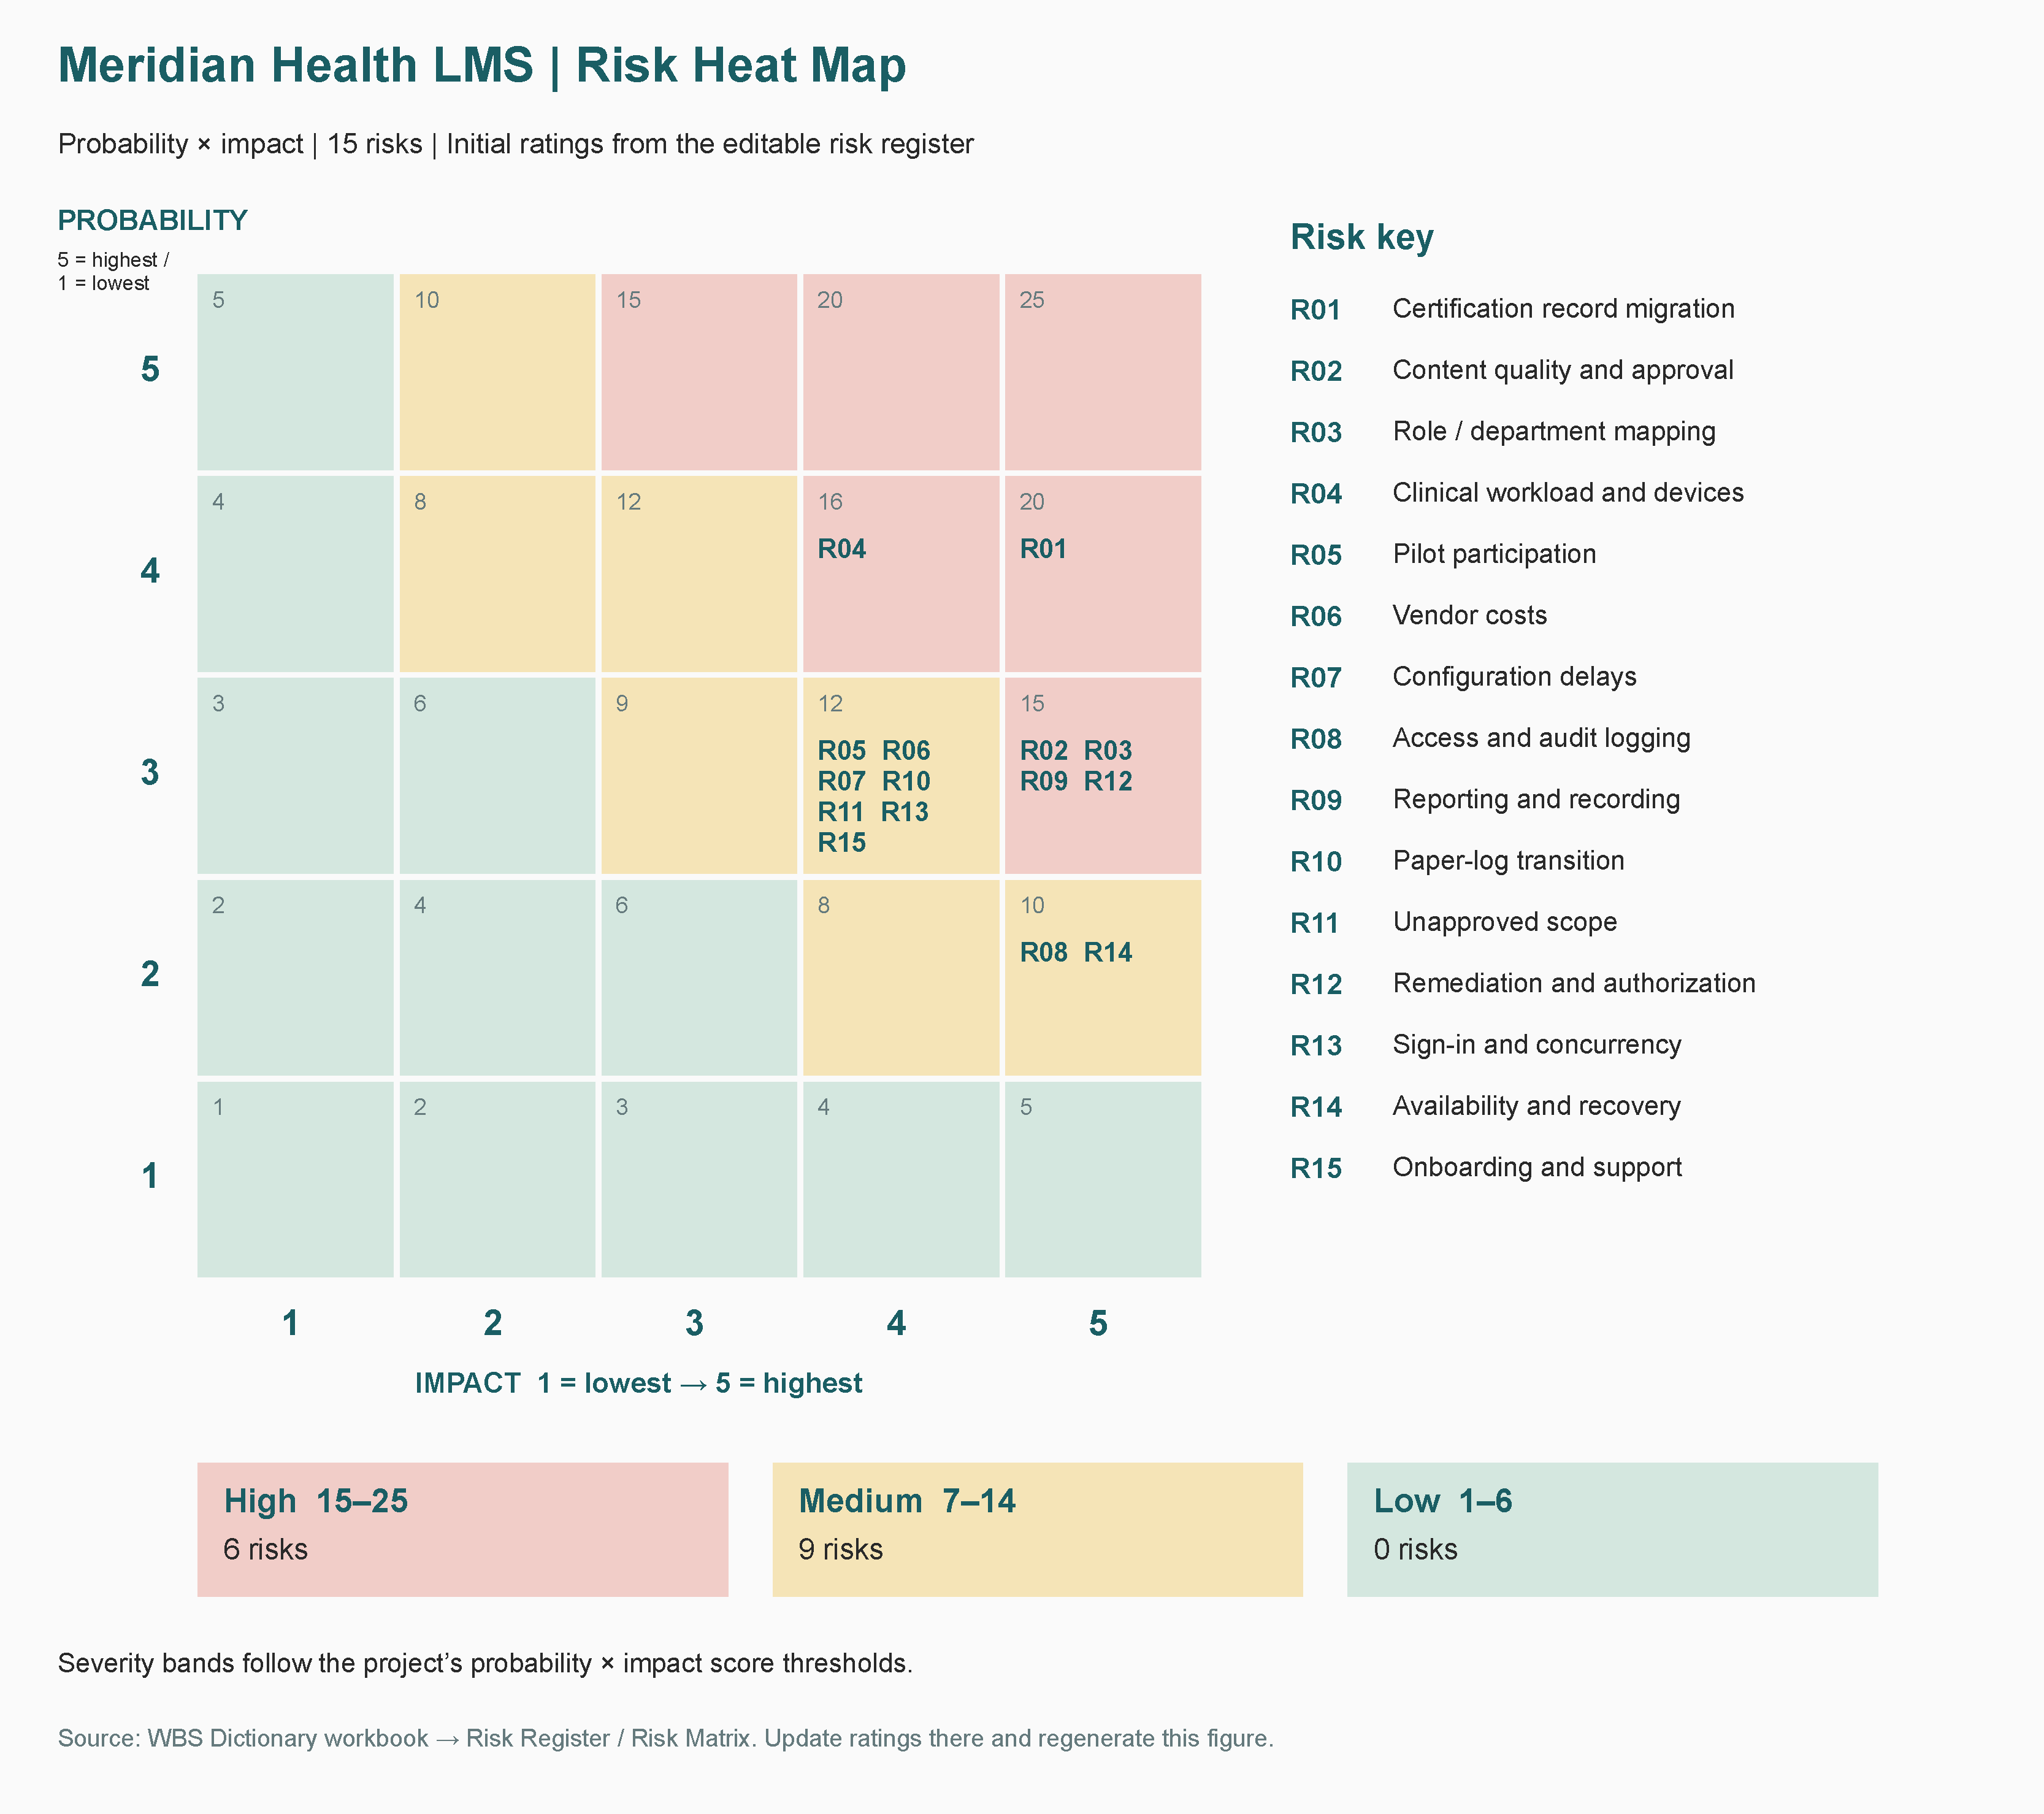
\includegraphics[width=0.78\textwidth,height=0.58\textheight,keepaspectratio]{figures/meridian_risk_matrix.pdf}%
  }{\fbox{\parbox[c][1.5in][c]{0.75\textwidth}{\centering
    Risk matrix placeholder. Upload \texttt{figures/meridian\_risk\_matrix.pdf}.}}}
  \caption{Probability/impact matrix for the Meridian Health LMS project.}
  \label{fig:risk-matrix}
\end{figure}

% ============================================================
% 5. COMMUNICATION MANAGEMENT PLAN
% ============================================================
\clearpage
\section{Communication Management Plan}

\subsection{Communication matrix}
% Recommended columns: Stakeholder group, Information needs, Frequency,
% Format, Owner/sender, Distribution method.
\placeholder{Insert the communication matrix from the Skeleton.}

\subsection{Status reporting}
\placeholder{Describe report frequency, distribution, contents, and status rules.}

\subsection{Meeting schedule}
% Recommended columns: Meeting, When, Duration, Attendees, Purpose.
\placeholder{Insert recurring meetings, stakeholder meetings, review/approval meetings, and meeting protocols.}

\subsection{Project documentation}
\placeholder{Describe storage, naming conventions, version control, access permissions, and retention.}

% ============================================================
% 6. QUALITY MANAGEMENT PLAN
% ============================================================
\clearpage
\section{Quality Management Plan}

\subsection{Quality standards}
\placeholder{Insert quality standards and deliverable-level acceptance criteria.}

\subsection{Quality assurance activities}
\subsubsection{Reviews and inspections planned}
\placeholder{Insert review schedule, reviewers, and outputs.}

\subsubsection{Testing approach}
\placeholder{Insert testing approach.}

\subsubsection{Validation methods}
\placeholder{Insert validation methods.}

\subsection{Quality control measures}
\subsubsection{Quality metrics and targets}
\placeholder{Insert metric, target, measurement method, timing, and owner.}

\subsubsection{Defect tracking approach}
\placeholder{Insert defect severity definitions, tracking method, and response.}

\subsubsection{Corrective action process}
\placeholder{Insert corrective action process.}

\end{document}
